%!TEX root = ../../super_main.tex

\section{Data Usefulness}
\label{sec:data_usefulness}

In order to test if the snapshot uMiner provides is useful for some reality mining related task we need investigate if it is possible to use the uMiner platform to gather snapshots to create some context aware application. We have for this reason created a simple campaign that asks the participants if their phone is placed on the table or not, corresponding to the specification shown in \tabref{tab:phone_placement_campaing}.

\begin{table}[!htbp]
    \centering
    \begin{tabular}{|m{0.34\textwidth}|m{0.6\textwidth}|} 
  \hline
  \textbf{Snapshot per Campaign}    & 30 snapshots      \\ \hline
  \textbf{Samples per Snapshot}     & 1 samples         \\ \hline
  \textbf{Sample delay}             & 4000 ms           \\ \hline
  \textbf{Measurement per Sample}   & 30 measurements   \\ \hline
  \textbf{Measurement delay}        & 200 ms            \\ \hline
  \textbf{Sensors}                  & \begin{itemize}[noitemsep]
                \item Accelerometer 
                \item Compass
                \item Gyroscope
              \end{itemize}                             \\ \hline
    \textbf{Questions}                & \begin{itemize}[noitemsep]
                                            \item Was the phone placed on the table?
                                        \end{itemize} \\ \hline
    \end{tabular}
    \caption{Phone placement campaign.}
    \label{tab:phone_placement_campaing}
\end{table}

As specified we only measure 1 sample per snapshot, and utilize $30 \cdot 200ms$  with a delay of $4000ms$ per sample, meaning that snapshots last 10 seconds. Note that a 10 second snapshot which is not seen as the average use case, since a question every 10 seconds is simply too intrusive for the participants in every scenario. Furthermore we have specified that we want 30 snapshots from this campaign, meaning that the participants of this campaign will be monitored for a 5 minute period in total. We have created this dense campaign simple because we wanted to get some snapshots we could quickly determine to be useful when creating some context aware application. The snapshots from this data was used to create an example application called \emph{Where Am I?} which will guess if the device is placed on the table or in the pocket, as seen in \figref{fig:where_am_i_app}.

\begin{figure}[!htbp]
    \centering
    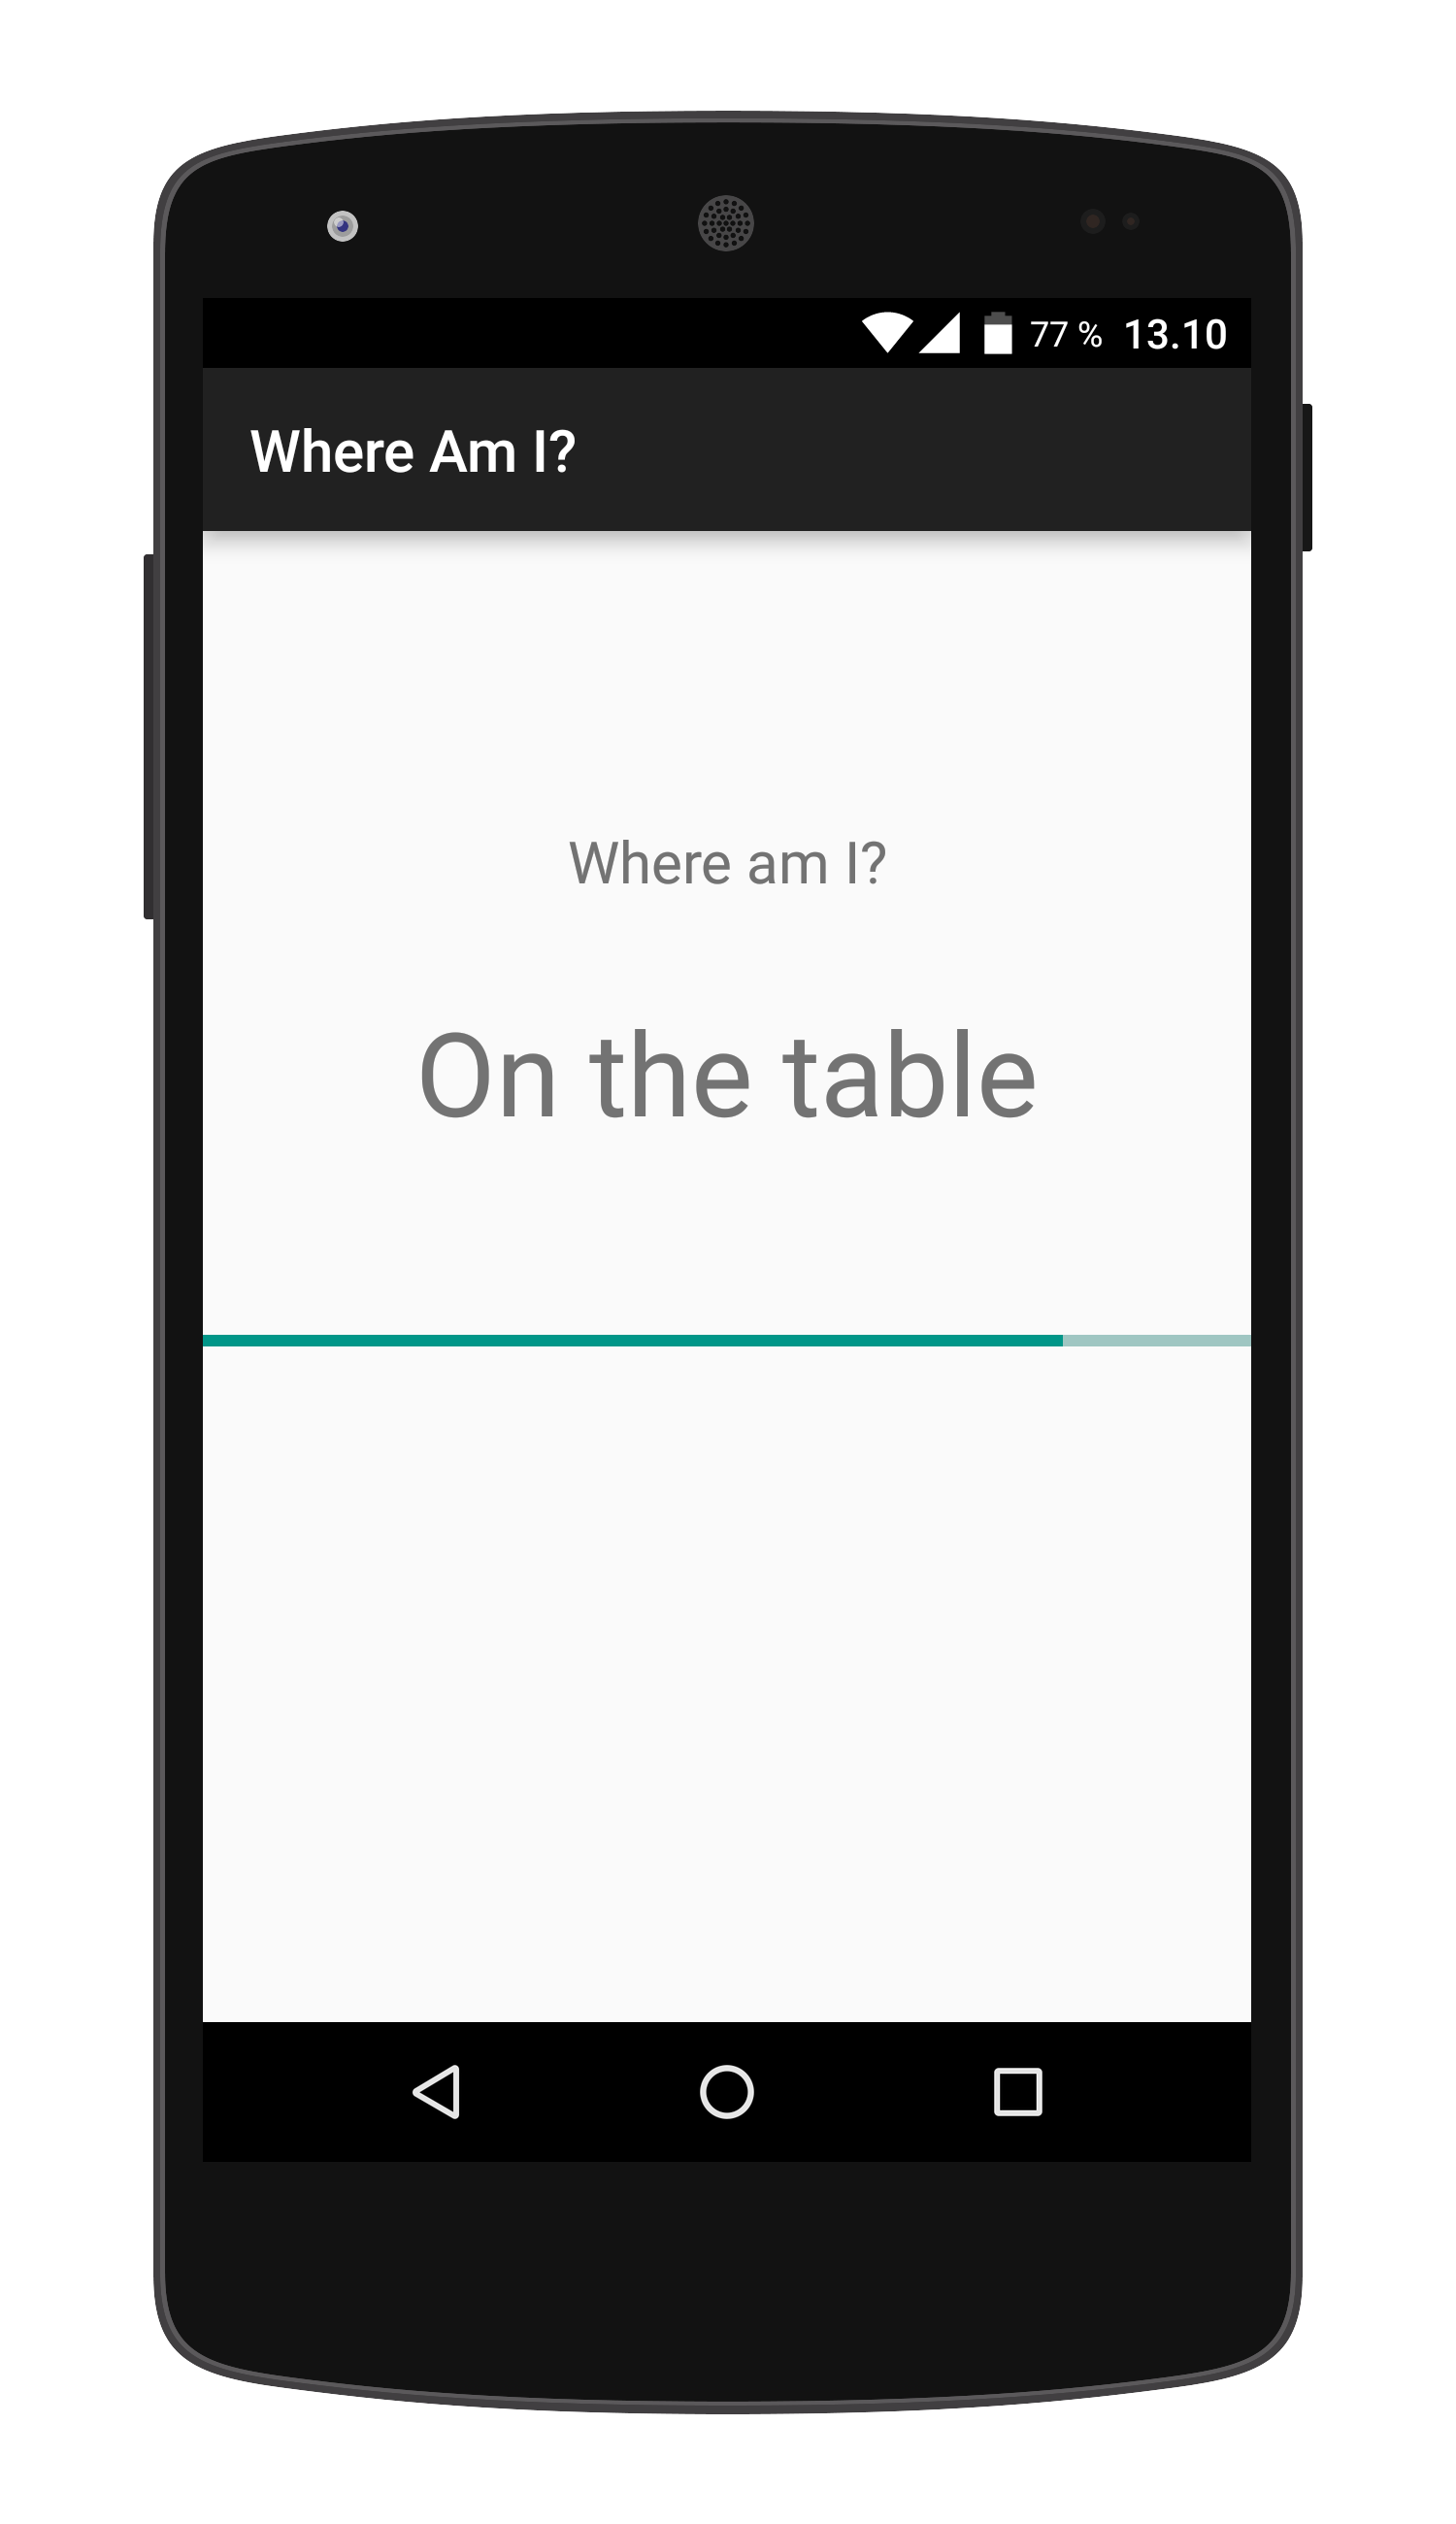
\includegraphics[width=.35\textwidth ]{graphic/quality_assurance/where_am_i_app.png}
    \caption{The example \emph{Where Am I?} application.}
    \label{fig:where_am_i_app}
\end{figure}
\FloatBarrier

The \emph{Where Am I?}-application will continuously guess if the phone is placed on a table or not using an underlying Naïve Bayes classifier. This application starts up, trains the classifier using the snapshots, and the predicts in real time the placement of the phone. This classifier was implemented using a library called WEKA\footnote{https://weka.wikispaces.com/}, which has some predefined methods and data types that makes it relatively easy to implement, and the gathering of sensor values is implemented using sensor providers from uMiner.
\\\\
Given our snapshot and a this machine intelligence model library, we found it pretty effortless to implement an application that have some notion of the context in which it exist. We only spend roughly 16 man hours on the creation and execution of campaign, and on features that allow this application to parse snapshots, train the model, display the prediction in a simple interface.